
% You need to select the LuaTeX engine to compile to pdf
% If you use Overleaf, you have to change the compiler (https://www.overleaf.com/learn/how-to/Changing_compiler)
% Reason: The common pdfTeX engine cannot use system fonts: Calibri, Georgia


\documentclass[aspectratio=169,smaller]{beamer}
%  aspect-ratios "43" and "169", and "smaller" or "9pt" should work

% Load package "amsmath" before PSI43 (because "fontspec" inside PSI43 should be loaded before "amsmath" according to an advice)
\usepackage{amsmath}

\usepackage[blockcolored, PSIitemize, PSIpageno]{PSI43} % blockcolored is required if you want to have colored blocks, because the default beamer theme has uncolored boxes


%% My personal suggestions:
% Remove the silly "Figure" in front of a figure caption in beamer:
\setbeamertemplate{caption}{\raggedright\insertcaption\par}
% The advice to use non-serif fonts for math was from a time
% where screen-resolution was low. With HD and UHD, this is obsolete IMHO.
\usefonttheme[onlymath]{serif} 

\begin{document}

\title{A novel approach to energy system analysis and technology assessment}

\author[L.~Wittgenstein]{Ludwig Wittgenstein}
% if short author is given as an option, it will be taken for the footline

\institute[LEA, PSI]{Laboratory of Energy Systems Analysis, Paul Scherrer Institute}
% if short institute is given as  an option, it will be taken for the footline

\subtitle{\textbf{Subtitle (different no of lines move the gray box at correct position. Empty line:  $\sim$\textbackslash\textbackslash)}}

\date{LEA Seminar, 1.1.2021} % can be left empty


\begin{frame}[plain] % plain prohibits logo, footer etc.
  \titlepage
\end{frame}


\begin{frame}[t]{A list that is revealed}
   \PSIvspace
  \begin{itemize}
  \item PSI-style itemize with option \texttt{PSIitemize}
  \item[--]  With dash instead of bullet
    \begin{enumerate}
    \item Enumerated 1a
    \item Enumerated 1b
    \end{enumerate}
    \pause
  \item Item 2 (revealed on next slide)
    \pause
  \item Item 3
    \begin{itemize}
    \item Item 4
      \begin{itemize}
      \item Item 5
      \end{itemize}
    \end{itemize}
  \end{itemize}
\end{frame}



\begin{frame}[squeeze]{Titles over two lines are possible\\
    (PSI logo goes to 2nd line)}
  Formulas can be algined and tagged, e.g.\ \thetag{$\ast$}:
  \begin{align*}
    \Gamma  & = \int_a^b f(x)\,dx             && \tag{$\ast$}\\
    \sum_{n=1}^N x_{i_n} &= \Bigl(\frac{a+b}{c+d}\Bigr)\cdot \sin(x)  &&
  \end{align*}
  \begin{itemize}
  \item  $\alpha = \zeta$; with \texttt{\textbackslash boldsymbol}: $\boldsymbol{\alpha} = \boldsymbol{\zeta}$ 
  \item $\mathcal{F}_t$, $\mathbb{R}^n$;  \texttt{\textbackslash to, iff, implies}: $f\colon X\to Y$, $A\iff B$, $A\implies B$
  \item Fine tuning of spacing: $\{t | t=1,\dots,T\}$ versus  $\{t \mid t=1,\dots,T\}$
  \item Fine tuning of spacing: $f: x\mapsto y$ versus $f\colon x\mapsto y$
  \item Fine tuning of spacing: $y_n x_n^m$ versus $y_n^{}x_n^m$
  \end{itemize}
   \alert{This is a frame with the usual `squeeze' option of beamer to narrow linespacing a little bit; the color of this text is called \texttt{alert} in beamer}
  
  \structure{This is a color predefined in beamer called \texttt{structure}}
\end{frame}

\begin{frame}[t]{Columns and Blocks}
\setbeamercolor{mycolor}{bg=PSIverylightgray}

You can start text high with a top-aligned frame in beamer

 The default beamer theme has uncolored blocks. The option \texttt{blockcolored} was set in the package for coloring: 
  \begin{columns}
    \column[T]{.5\linewidth}
      \begin{block}{Title of block}
        Top-aligned block in first column
      \end{block}
      \begin{exampleblock}{Title of example block}
        Block in first column
      \end{exampleblock}
      Text outside of block in first column
      \vspace{1ex}
      
      \begin{beamercolorbox}[wd=\linewidth, colsep*=4pt]{mycolor}
         This is a box (without title)
       \end{beamercolorbox}
   \column[T]{.4\linewidth}
      \begin{block}{Title in block}
        Block in second column 
      \end{block}
      \begin{alertblock}{Title of alert block}
        Block in second column
      \end{alertblock}
      \begin{block}{}
        Block with empty title
      \end{block}
    \end{columns}
    
    \vspace{1ex}
    \begin{beamercolorbox}[wd=\linewidth, colsep*=4pt]{mycolor}
      This is a box (without title)
    \end{beamercolorbox}
 \end{frame}
 

 \begin{frame}[t]{Title}
   \PSIvspace
  You can start text at the gray box with the command \texttt{\textbackslash PSIspace} and a top-aligned frame in beamer (see the .tex file)
  \begin{figure}
    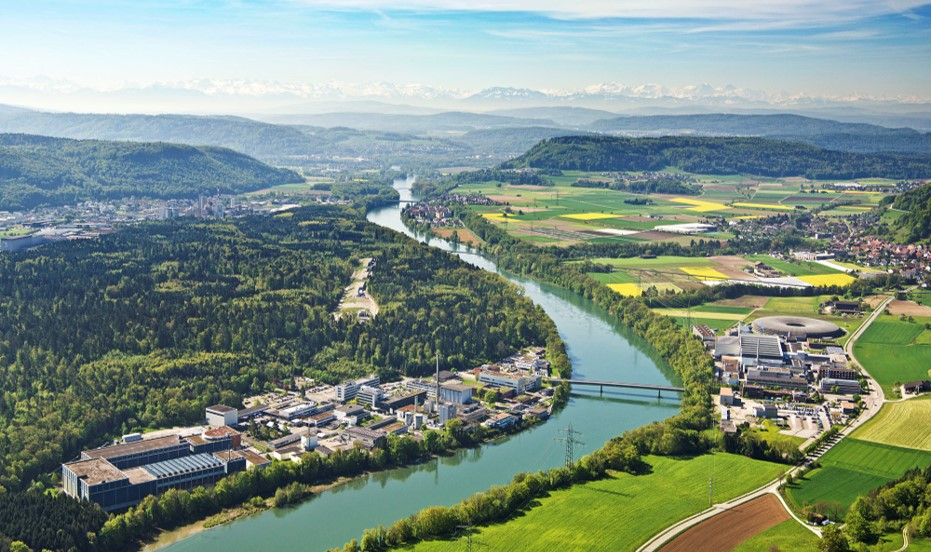
\includegraphics[width=0.3\pagewidth]{PSIlandscape43}
    \caption{Figures are automatically centered in beamer}
    \label{fig:PSI}
  \end{figure}
\end{frame}

\begin{frame}[t]{Overwrite the margins}
  You can overwrite the margins with a wide column:
  \setbeamercolor{mycolor}{fg=PSIgray, bg=structure!10}
\begin{columns}
  \column{1.1\linewidth}
    We need more space:
  \begin{beamercolorbox}[wd=\textwidth, dp=0.7\textheight, colsep*=4pt]{mycolor}
    This is a very long text that needs a lot of space this is a very long text that needs a lot of space this is a very long text that needs a lot of space
  \end{beamercolorbox}
\end{columns}
\end{frame}

\PSItrailer{Wir schaffen Wissen -- heute für morgen}{
    \textbf{My thanks go to}
     \smallskip
    \begin{itemize}
    \item Co-author 1
    \item Co-author 2 who has a very long name 
    \item Supervisor 1
    \item Supervisor 2  
    \end{itemize}
    }
  

\end{document}

% The following can be deleted if not the EMACS editor is used for editing

%%%Local Variables:
%%% mode: latex
%%% TeX-master: t
%%% TeX-engine: luatex
%%% End:
